\chapter{Performance Measurements} \label{appendix-performance}
\captionsetup{margin=10pt,font=large,labelfont=bf,textfont={bf}}

\begin{figure}[h]
	\centering
	\captionof{table}{{\large \textbf{Non-Progressive Algorithms by Number of Tuples}}}
	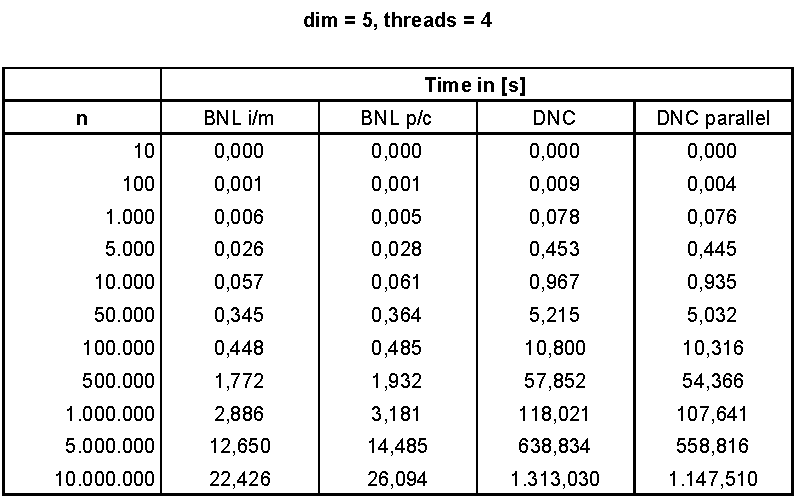
\includegraphics[width=0.9\linewidth]{figures/table-non-progressive-n}
	\label{fig:table-non-progressive-n}
\end{figure}

\begin{figure}[H]
	\centering
	\captionof{table}{Non-Progressive Algorithms by Dimensionality}
	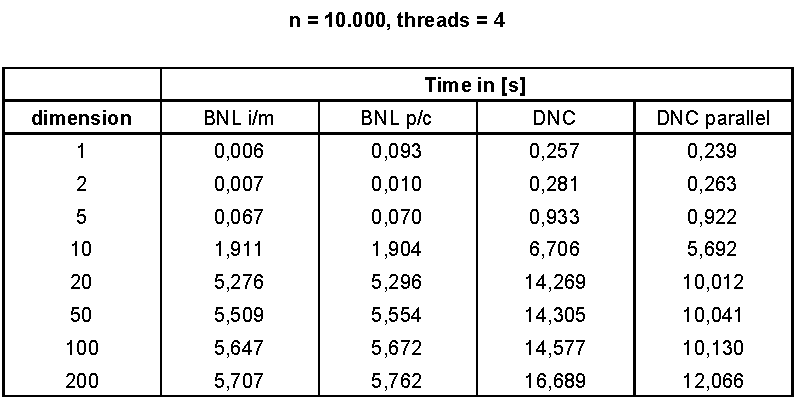
\includegraphics[width=0.9\linewidth]{figures/table-non-progressive-dim}
	\label{fig:table-non-progressive-dim}
\end{figure}

\begin{figure}[h]
	\centering
	\captionof{table}{Non-Progressive Algorithms by Number of Threads}
	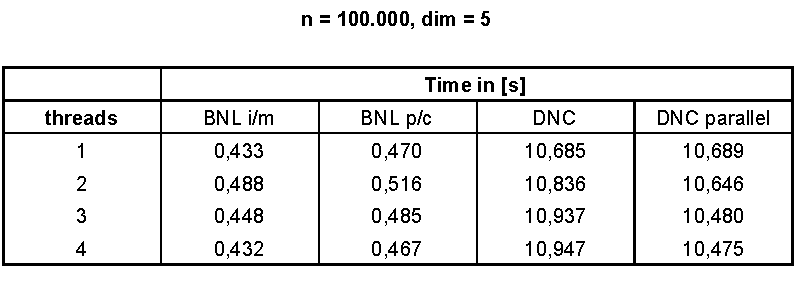
\includegraphics[width=0.9\linewidth]{figures/table-non-progressive-threads}
	\label{fig:table-non-progressive-threads}
\end{figure}

\begin{figure}[H]
	\centering
	\captionof{table}{Progressive Algorithms by Number of Tuples}
	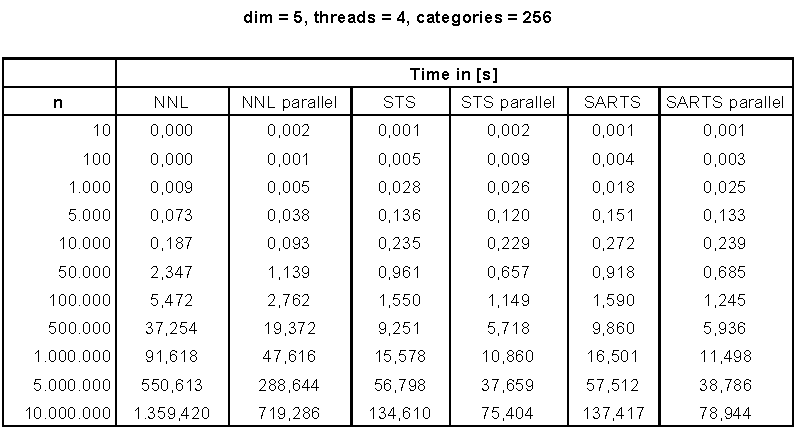
\includegraphics[width=1\linewidth]{figures/table-progressive-n}
	\label{fig:table-progressive-n}
\end{figure}

\begin{figure}[h]
	\centering
	\captionof{table}{Progressive Algorithms by Dimensionality}
	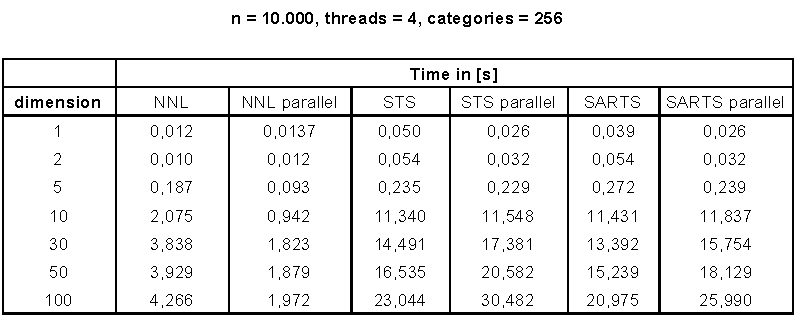
\includegraphics[width=1\linewidth]{figures/table-progressive-dim}
	\label{fig:table-progressive-dim}
\end{figure}

\begin{figure}[h]
	\centering
	\captionof{table}{Progressive Algorithms by Number of Threads}
	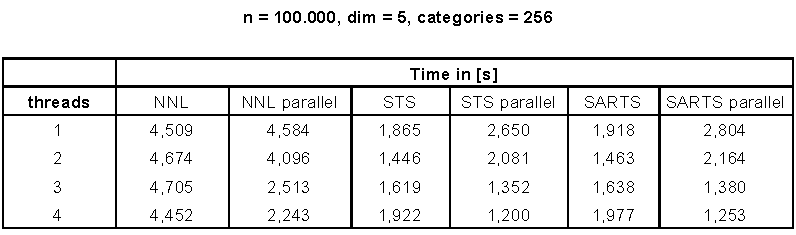
\includegraphics[width=1\linewidth]{figures/table-progressive-threads}
	\label{fig:table-progressive-threads}
\end{figure}

\begin{figure}[H]
	\centering
	\captionof{table}{Memory Usage by Number of Tuples}
	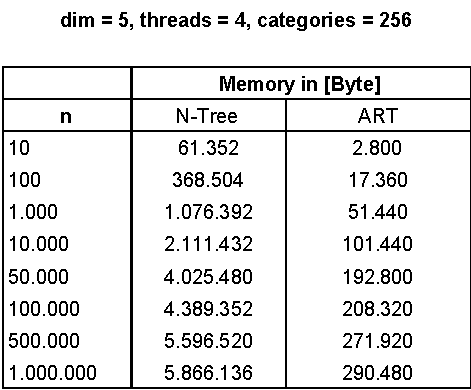
\includegraphics[width=0.53\linewidth]{figures/table-memory-usage-n}
	\label{fig:table-memory-usage-n}
\end{figure}

\begin{figure}[H]
	\centering
	\captionof{table}{Memory Usage by Dimensionality}
	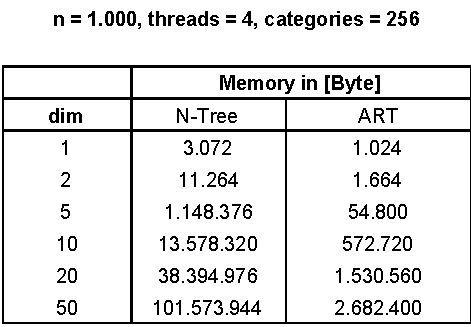
\includegraphics[width=0.55\linewidth]{figures/table-memory-usage-dim}
	\label{fig:table-memory-usage-dim}
\end{figure}



\chapter{C++ Code} \label{appendix-code}
\usemintedstyle{bw}

\section{Dominates Operation for NNL, BNL and DNC}
\begin{minted}[tabsize=3,breaklines,fontsize=\small]{c++}
/**
* Checks whether one tuple dominates the other and returns true|false
* @param dominator the tuple to check for dominating
* @param dominated the tuple to check for being dominated
*/
bool dominates(const std::vector<int> &dominator, const std::vector<int> &dominated){
	bool flag = true;
	for(std::vector<int>::size_type i = 0; i< dominated.size(); i++){
		if(dominator[i] > dominated[i]) return false;
		if(dominated[i] > dominator[i]) flag = false;
	}
	if(flag) return false;
	return true;
}
\end{minted}

\section{Naive-Nested-Loops}
\begin{minted}[tabsize=3,breaklines,fontsize=\small]{c++}
void computeSkylineProduce(){
	for(std::size_t i = 0; i < storage.size(); i++){
		bool not_dominated = true;
		for(std::size_t j = 0; j < storage.size(); j++){
			if(i != j){
				if(dominates(storage[j], storage[i])){
					not_dominated = false;
					break;
				}
			}
		}
		if(not_dominated){
			parent->consume(storage[i]);
		}
	}
}
\end{minted}

\section{Naive-Nested-Loops Parallelized}
\begin{minted}[tabsize=3,breaklines,fontsize=\small]{c++}
void computeSkylineProduceParallel(){
	const std::vector<std::vector<int>> storage = this->storage;
	CatOperator *parent = this->parent;
	parallel_for(std::size_t(0), storage.size(), [this, storage, parent]( std::size_t i ) {
		bool not_dominated = true;
		bool flag = false;
		for(std::size_t j = 0; j < storage.size() && !flag; j++){
			if(i != j){
				if(dominates(storage[j], storage[i])){
					not_dominated = false;
					flag = true;
				}
			}
		}
		// The following mutex slows down the parallelization, but provides an easy way to avoid race conditions
		// In case no mutex is used, the programmer needs to make sure that no race condition occurs in the following if-block
		static spin_mutex mtx;
		spin_mutex::scoped_lock lock(mtx);
		if(not_dominated){
			parent->consume(storage[i]);
		}
	} );
}
\end{minted}

\section{Block-Nested-Loops Volcano Model}
\begin{minted}[tabsize=3,breaklines,fontsize=\small]{c++}
void computeSkyline(){
	// storage is the window here
	storage.push_back(child->getNext());
	while(true){
		std::vector<int> tuple = child->getNext();
		if(!tuple.empty()){
			storage.push_back(tuple);
			for(std::size_t j = 0; j < storage.size()-1; j++){
				if(dominates(storage.back(), storage[j])){
					storage.erase(storage.begin() + j);
					j--;
				}
				else if (dominates(storage[j], storage.back())){
					storage.erase(storage.begin() + storage.size()-1);
					break;
				}
			}
		}
		else break;
	}
}
\end{minted}

\section{Block-Nested-Loops Produce/Consume}
\begin{minted}[tabsize=3,breaklines,fontsize=\small]{c++}
void computeSkylineProduce(){
	// storage contains tuples produced by the generator
	std::vector<std::vector<int>> window;
	window.push_back(storage[0]);
	for(std::size_t i = 1; i < storage.size(); i++){
		std::vector<int> tuple = storage[i];
		window.push_back(tuple);
		for(std::size_t j = 0; j < window.size()-1; j++){
			if(dominates(window.back(), window[j])){
				window.erase(window.begin() + j);
				j--;
			}
			else if (dominates(window[j], window.back())){
				window.erase(window.begin() + window.size()-1);
				break;
			}
		}
	}
	for(std::size_t i = 0; i < window.size(); i++){
		parent->consume(window[i]);
	}
}
\end{minted}

\section{Divide-and-Conquer}

\subsubsection{{\large Algorithm}}
\begin{minted}[tabsize=3,breaklines,fontsize=\small]{c++}
std::vector<std::vector<double>> computeSkyline(const std::vector<std::vector<double>> &M, const int &dimension){
	if(M.size() == 1) return M;
	
	std::vector<double> pivot = median(M, dimension-1); // dimension-1 because we need the last index
	std::pair<std::vector<std::vector<double>>, std::vector<std::vector<double>>> P = partition(M, dimension-1, pivot);
	
	std::vector<std::vector<double>> S_1, S_2;
	S_1 = computeSkyline(P.first, dimension);
	S_2 = computeSkyline(P.second, dimension);
	
	std::vector<std::vector<double>> result;
	std::vector<std::vector<double>> merge_result = mergeBasic(S_1, S_2, dimension);
	
	// Union S_1 and merge_result
	for(std::vector<std::vector<double>>::size_type i = 0; i < S_1.size(); i++){
		result.push_back(S_1[i]);
	}
	for(std::vector<std::vector<double>>::size_type i = 0; i < merge_result.size(); i++){
		result.push_back(merge_result[i]);
	}
	
	return result;
}
\end{minted}

\subsubsection{{\large Partition Operation}}
\begin{minted}[tabsize=3,breaklines,fontsize=\small]{c++}
std::pair<std::vector<std::vector<double>>, std::vector<std::vector<double>>> partition(const std::vector<std::vector<double>> &tuples, const int &dimension, const std::vector<double> &pivot){
	std::vector<std::vector<double>> P_1, P_2;
	std::pair<std::vector<std::vector<double>>, std::vector<std::vector<double>>> partitions;
	
	for(std::vector<std::vector<double>>::size_type i = 0; i < tuples.size(); i++){
		if(tuples[i][dimension] < pivot[dimension])
			P_1.push_back(tuples[i]);
		else
			P_2.push_back(tuples[i]);
	}
	
	partitions.first = P_1;
	partitions.second = P_2;
	
	return partitions;
}
\end{minted}
\subsubsection{{\large Merge Operation}}
\begin{minted}[tabsize=3,breaklines,fontsize=\small]{c++}
std::vector<std::vector<double>> mergeBasic(std::vector<std::vector<double>> S_1, const std::vector<std::vector<double>> &S_2, const int &dimension){
	std::vector<std::vector<double>> result;
	
	if(S_2.size() == 0) return result;
	
	if(S_1.size() == 1){ // trivial case - S_1 has only 1 tuple
		for(std::vector<std::vector<double>>::size_type i = 0; i < S_2.size(); i++){
			if(!dominates(S_1[0], S_2[i]))
				result.push_back(S_2[i]);
		}
	}
	else if(S_2.size() == 1){ // trivial case - S_2 has only 1 tuple
		result.push_back(S_2[0]);
		for(std::vector<std::vector<double>>::size_type i = 0; i < S_1.size(); i++){
			if(dominates(S_1[i], S_2[0])){
				result.erase(result.begin());
				break;
			}
		}
	}
	else if(S_1[0].size() == 2){ // low dimension
		// Min from S_1 according to dimension 1
		std::sort(S_1.begin(), S_1.end(), [](const std::vector<double> &a, const std::vector<double> &b){
			return a[0] < b[0];
		});
		std::vector<double> min = S_1[0];
		// Compare S_2 to Min according to dimension 1; in dimension 2 S_1 is always better
		for(std::vector<std::vector<double>>::size_type i = 0; i < S_2.size(); i++){
			if(S_2[i][0] < min[0]) result.push_back(S_2[i]);
		}
	}
	else{ // general case
		std::vector<double> pivot = median(S_1, dimension-1-1);
		std::pair<std::vector<std::vector<double>>, std::vector<std::vector<double>>> partitions_dim_1 = partition(S_1, dimension-1-1, pivot);
		std::pair<std::vector<std::vector<double>>, std::vector<std::vector<double>>> partitions_dim_2 = partition(S_2, dimension-1-1, pivot);
		std::vector<std::vector<double>> result_1, result_2, result_3;
		
		result_1 = mergeBasic(partitions_dim_1.first, partitions_dim_2.first, dimension);
		result_2 = mergeBasic(partitions_dim_1.second, partitions_dim_2.second, dimension);
		result_3 = mergeBasic(partitions_dim_1.first, result_2, dimension-1);
		
		// Union result_1 and result_3
		for(std::vector<std::vector<double>>::size_type i = 0; i < result_1.size(); i++){
			result.push_back(result_1[i]);
		}
		for(std::vector<std::vector<double>>::size_type i = 0; i < result_3.size(); i++){
			result.push_back(result_3[i]);
		}
	}
	
	return result;
}
\end{minted}

\section{ST-S/ SARTS}
\begin{minted}[tabsize=3,breaklines,fontsize=\small]{c++}
void computeSkylineProduce(){
	// pre-sort tuples in place
	sort(storage);
	std::vector<int> t_stop = storage[0];
	tree.insert(storage[0], tree.root, 0);
	parent->consume(storage[0]);
	for(std::size_t i = 1; i < storage.size(); i++){
		// stop if all the tuples left are dominated à-priori
		if((max(t_stop) <= min(storage[i])) && (t_stop != storage[i])){
			return;
		}
		// check for dominance
		if(!tree.is_dominated(storage[i], tree.root, 0, tree.score(storage[i]))){
			parent->consume(storage[i]);
			tree.insert(storage[i], tree.root, 0);
			if(max(storage[i]) < max(t_stop)){
				t_stop = storage[i];
			}
		}
	}
}
\end{minted}

\section{ST-S/ SARTS Parallelized}

\subsubsection{{\large Algorithm}}
\begin{minted}[tabsize=3,breaklines,fontsize=\small]{c++}
void computeSkylineProduce(){
	const std::vector<std::vector<int>> storage = this->storage;
	const std::size_t number_of_threads = NUMBER_OF_THREADS;
	std::vector<Tree*> subtrees;
	for(std::size_t i = 0; i < NUMBER_OF_THREADS; i++){
		Tree* subtree = new Tree(tree.get_attributes());
		subtrees.push_back(subtree);
	}
	std::future<void> futures[NUMBER_OF_THREADS];	
	// compute subquery skylines
	for(std::size_t i = 0; i < number_of_threads; i++){
		std::vector<std::vector<int>> subset;
		if(i == number_of_threads-1){
			subset.resize(storage.size() / number_of_threads + storage.size() % number_of_threads);
		}
		else{
			subset.resize(storage.size() / number_of_threads);
		}
		for(std::size_t j = 0; j < subset.size(); j++){
			subset[j] = storage[i*(storage.size()/number_of_threads) + j];
		}
		// Replace &ParallelSTS by &ParallelSARTS to receive SARTS
		futures[i] = std::async(std::launch::async, &ParallelSTS::computeSkylineSubset, this, i, subset, subtrees[i]);
	}
	for(std::size_t i = 0; i < NUMBER_OF_THREADS; i++){
		futures[i].get();
	}	
	// compute final skyline
	std::vector<std::vector<int>> input;
	for(std::size_t i = 0; i < subset_results.size(); i++){
		if(!subset_results[i].empty()){
			input.push_back(subset_results[i]);
		}
	}
	sort(input);
	std::vector<int> t_stop = input[0];
	tree.insert(input[0], tree.root, 0);
	parent->consume(input[0]);
	for(std::size_t i = 1; i < input.size(); i++){
		if((max(t_stop) <= min(input[i])) && (t_stop != input[i])){
			return;
		}
		if(!ntree.is_dominated(input[i], tree.root, 0, tree.score(input[i]))){
			parent->consume(input[i]);
			tree.insert(input[i], tree.root, 0);
			if(max(input[i]) < max(t_stop)){
				t_stop = input[i];
			}
		}
	}
	// free memory
	for(std::size_t i = 0; i < subtrees.size(); i++){
		if(subtrees[i] != nullptr) delete subtrees[i];
	}
}
\end{minted}
\subsubsection{{\large ComputeSkylineSubset Operation}}
\begin{minted}[tabsize=3,breaklines,fontsize=\small]{c++}
void computeSkylineSubset(unsigned threadNumber, std::vector<std::vector<int>> tuples, Tree* tree){
	// pre-sort tuples in place
	sort(tuples);
	std::vector<int> t_stop = tuples[0];
	tree->insert(tuples[0], tree->root, 0);
	subset_results[threadNumber * (subset_results.size() / NUMBER_OF_THREADS) + 0] = tuples[0];
	for(std::size_t k = 1; k < tuples.size(); k++){
		// stop if all tuples left are dominated a-priori
		if((max(t_stop) <= min(tuples[k])) && (t_stop != tuples[k])){
			return;
		}
		// check for dominance
		if(!tree->is_dominated(tuples[k], tree->root, 0, tree->score(tuples[k]))){
			subset_results[threadNumber * (subset_results.size() / NUMBER_OF_THREADS) + k] = tuples[k];
			tree->insert(tuples[k], tree->root, 0);
			if(max(tuples[k]) < max(t_stop)){
				t_stop = tuples[k];
			}
		}
	}
}
\end{minted}

\section{N-Tree}

\subsubsection{{\large Insert Operation}}
\begin{minted}[tabsize=3,breaklines,fontsize=\small]{c++}
void NTree::insert(const std::vector<int> &tuple, node* p, unsigned int level){
	if(level == 0){
		p->minScore = 0;
		p->maxScore = 0;
		for(std::size_t i = 0; i < tuple.size(); i++){
			p->maxScore += (int) (pow(2.0, (double) (tuple.size()-i)) * attributes[attributes.size()-1]);
		}
	}
	else{
		p->minScore = 0;
		for(std::size_t i = 0; i < level; i++){
			p->minScore += (int) (pow(2.0, (double) (tuple.size()-i)) * tuple[i]);
		}
		p->maxScore = p->minScore;
		for(std::size_t i = level; i < tuple.size(); i++){
			p->maxScore += (int) (pow(2.0, (double) (tuple.size()-i)) * attributes[attributes.size()-1]);
		}
	}
	if(level == tuple.size()){
		p->tupleIDs.push_back(tupleID++);
	}
	else{
		if(p->children.empty()){
			p->children.resize(attributes.size());
		}
		if(!p->children[tuple[level]]){
			p->children[tuple[level]]=new node();
		}
		insert(tuple, p->children[tuple[level]], level+1);
	}
}
\end{minted}

\subsubsection{{\large Is\_Dominated Operation}}
\begin{minted}[tabsize=3,breaklines,fontsize=\small]{c++}
bool NTree::is_dominated(const std::vector<int> &tuple, node* p, unsigned int level, unsigned int currentScore){
	if(p==nullptr || (currentScore < p->minScore)){
		return false;
	}
	if((level == tuple.size()) && (score(tuple) != p->minScore)){
		return true;
	}
	if((level == tuple.size()) && (score(tuple) == p->minScore)){
		return false;
	}
	// search the subtrees from left to right
	unsigned int weight = (int) (pow(2.0, (double) (tuple.size()-level)) * tuple[level]);
	for(int i = 0; i < tuple[level]; i++){
		if(is_dominated(tuple, p->children[i], level+1, currentScore + weight)){
			return true;
		}
	}
	if(is_dominated(tuple, p->children[tuple[level]], level+1, currentScore)){
		return true;
	}
	return false;
}
\end{minted}

\section{ART}
%\subsection{Nodes}

\subsubsection{{\large Insert Operation}}
\begin{minted}[tabsize=3,breaklines,fontsize=\small]{c++}
void ART::insert(const std::vector<int> &tuple, Node *&parent, Node *&current, unsigned int level){
	if(level == 0){
		current->minScore = 0;
		current->maxScore = 0;
		for(std::size_t i = 0; i < tuple.size(); i++){
			current->maxScore += (int) (pow(2.0, (double) (tuple.size()-i)) * attributes[attributes.size()-1]);
		}
	}
	else{
		current->minScore = 0;
		for(std::size_t i = 0; i < level; i++){
			current->minScore += (int) (pow(2.0, (double) (tuple.size()-i)) * tuple[i]);
		}
		current->maxScore = current->minScore;
		for(std::size_t i = level; i < tuple.size(); i++){
			current->maxScore += (int) (pow(2.0, (double) (tuple.size()-i)) * attributes[attributes.size()-1]);
		}
	}
	if(level == tuple.size()){
		current->tupleIDs.push_back(tupleID++);
	}
	else{
		Node* child = findChild(current, tuple[level]);
		if(!child){
			switch(current->type){
				case NodeType4:
					if(current->count == 4) 
						grow(parent, current, tuple[level-1]);
					break;
				case NodeType16:
					if(current->count == 16) 
						grow(parent, current, tuple[level-1]);
					break;
				case NodeType48:
					if(current->count == 48) 
						grow(parent, current, tuple[level-1]);
					break;
				case NodeType256:
				default:
					break;
			}
			child = newChild(current, tuple[level]);
		}
		insert(tuple, current, child, level+1);
	}
}
\end{minted}

\subsubsection{{\large Is\_Dominated Operation}}
\begin{minted}[tabsize=3,breaklines,fontsize=\small]{c++}
bool ART::is_dominated(const std::vector<int> &tuple, Node* p, unsigned int level, unsigned int currentScore){
	if(p==NULL || (currentScore < p->minScore)){
		return false;
	}
	if((level == tuple.size()) && (score(tuple) != p->minScore)){
		return true;
	}
	if((level == tuple.size()) && (score(tuple) == p->minScore)){
		return false;
	}
	// search the subtrees from left to right
	unsigned int weight = (int) (pow(2.0, (double) (tuple.size()-level)) * tuple[level]);
	for(int i = 0; i < tuple[level]; i++){
		Node* child = findChild(p, i);
		if(child){ // if child not null
			if(is_dominated(tuple, child, level+1, currentScore + weight)){
				return true;
			}
		}
	}
	Node* child = findChild(p, tuple[level]);
	if(child){
		if(is_dominated(tuple, child, level+1, currentScore)){
			return true;
		}
	}
	return false;
}
\end{minted}

\subsubsection{{\large Find\_Child Operation}}
\begin{minted}[tabsize=3,breaklines,fontsize=\small]{c++}
Node* ART::findChild(Node* parent, const int &attribute){
	switch(parent->type){
		case NodeType4: {
			Node4* node = static_cast<Node4*>(parent);
			for (unsigned i = 0; i < node->count; i++){
				if (node->key[i] == attribute){
					return node->children[i];
				}
			}
			return NULL;
		}
		case NodeType16: {
			Node16* node = static_cast<Node16*>(parent);
			for (unsigned i = 0; i < node->count; i++){
				if (node->key[i] == attribute){
					return node->children[i];
				}
			}
			return NULL;
		}
		case NodeType48: {
			Node48* node = static_cast<Node48*>(parent);
			if (node->childIndex[attribute] != emptyMarker){
				return node->children[node->childIndex[attribute]];
			}
			else
				return NULL;
		}
		case NodeType256: {
			Node256* node = static_cast<Node256*>(parent);
			return node->children[attribute];
		}
		default: {
			return NULL;
		}
	}
}
\end{minted}

\subsubsection{{\large New\_Child Operation}}
\begin{minted}[tabsize=3,breaklines,fontsize=\small]{c++}
Node* ART::newChild(Node *&node, const int &attribute){
	Node4* child = new Node4();
	switch(node->type){
		case NodeType4: {
			Node4* parent = static_cast<Node4*>(node);
			unsigned pos;
			// make free space for the new child entry
			for (pos = 0; (pos < parent->count) && (parent->key[pos] < attribute); pos++);
			memmove(parent->key+pos+1, parent->key+pos, parent->count-pos);
			memmove(parent->children+pos+1, parent->children+pos, (parent->count-pos)*sizeof(Node*));
			parent->key[pos] = attribute;
			parent->children[pos] = child;
			parent->count++;
			break;
		}
		case NodeType16: {
			Node16* parent = static_cast<Node16*>(node);
			unsigned pos;
			// make free space for the new child entry
			for (pos = 0; (pos < parent->count) && (parent->key[pos] < attribute); pos++);
			memmove(parent->key+pos+1, parent->key+pos, parent->count-pos);
			memmove(parent->children+pos+1, parent->children+pos, (parent->count-pos)*sizeof(Node*));
			parent->key[pos] = attribute;
			parent->children[pos] = child;
			parent->count++;
			break;
		}
		case NodeType48: {
			Node48* parent = static_cast<Node48*>(node);
			unsigned pos = parent->count;
			// if there are empty slots inbetween, use them instead of appending the child pointer at the end
			if(parent->children[pos]){
				for(pos = 0; parent->children[pos] != NULL; pos++);
			}
			parent->children[pos] = child;
			parent->childIndex[attribute] = pos;
			parent->count++;
			break;
		}
		case NodeType256: {
			Node256* parent = static_cast<Node256*>(node);
			parent->children[attribute] = child;
			parent->count++;
			break;
		}
		default:
			break;
	}
	return child;
}
\end{minted}

\subsubsection{{\large Grow Operation}}
\begin{minted}[tabsize=3,breaklines,fontsize=\small]{c++}
void ART::grow(Node *&parent, Node *&node, const int &indexOfCurrent){
	Node* newNode;
	switch(node->type){
		case NodeType4:
			newNode = new Node16();
			newNode->count = 4;
			for(std::size_t i = 0; i < 4; i++){
				static_cast<Node16*>(newNode)->key[i] = static_cast<Node4*>(node)->key[i];
			}
			for(std::size_t i = 0; i < 4; i++){
				static_cast<Node16*>(newNode)->children[i] = static_cast<Node4*>(node)->children[i];
			}
			break;
		case NodeType16:
			newNode = new Node48();
			newNode->count = 16;
			for(std::size_t i = 0; i < 16; i++){
				static_cast<Node48*>(newNode)->children[i] = static_cast<Node16*>(node)->children[i];
			}
			for (unsigned i = 0; i < node->count; i++){
				static_cast<Node48*>(newNode)->childIndex [static_cast<Node16*>(node)->key[i]] = i;
			}
			break;
		case NodeType48:
			newNode = new Node256();
			newNode->count = 48;
			for (unsigned i = 0; i < 256; i++){
				if (static_cast<Node48*>(node)->childIndex[i] != 48){ // slot not empty
					static_cast<Node256*>(newNode)->children[i] = static_cast<Node48*>(node)->children [static_cast<Node48*>(node)->childIndex[i]];
				}
			}
			break;
		default:
			break;
	}
	newNode->minScore = node->minScore;
	newNode->maxScore = node->maxScore;
	for(std::size_t i = 0; i < node->tupleIDs.size(); i++){
		newNode->tupleIDs[i] = node->tupleIDs[i];
	}
	
	if(node != root){
		// Code to updateParent() is not given for space reasons. Contact the author if needed. 
		updateParent(parent, newNode, indexOfCurrent);
	}
	delete node;
	node = newNode;
}
\end{minted}







